\section{Auswertung}
\label{sec:Auswertung}

\subsection{Brechungsindex über die senkrechte Polarisation}
Zu erst wird die Fresnel Formel \eqref{eq:1} nach n umgestellt. Dadurch ergibt sich 
\begin{equation}
  n=\sqrt{1+\frac{4E_{\bot}\cos^2{\alpha}}{(E_{\bot}-1)^2}}
  \label{ns}
\end{equation}
für $n$, mit $E_{\bot}=\sqrt{\frac{I_r-I_d}{I_e-I_d}}$, wobei $I_r$ der gemessene Strom des reflektierten Lasers, $I_e$ der einfallende Strom des Lasers und $I_d$ der Dunkelstrom ist. Einsetzen der Messwerte für die jeweiligen Winkel in \eqref{ns} und einsetzen dieser in
\begin{equation}
  \bar n=\frac{1}{N}\sum n_i
  \label{m}
\end{equation}
ergibt mit Python den Mittelwert 
\begin{equation*}
  \bar n=2.53 \pm 0.18,
\end{equation*}
wobei der Fehler mit
\begin{equation}
  \Delta n=\sqrt{\frac{1}{N(N-1)}\sum (n_i-\bar n)^2}
  \label{f}
\end{equation}
berechnet wurde. Die zu den Winkeln gemessenen Stromwerte, Amplitudenverhätlnisse und berechneten Brechungsindizes befinden sich in \autoref{i1}. 
\begin{table}[H]
  \centering
  \caption{Winkel, gemessene Stromwerte, Amplitudenverhältnisse und Brechungsindizes für den senkrechten Fall.}
  \begin{tabular}{l|l|l|l|l|l|l|l}
  Winkel/° & $I_r$/$\mu$A & $E_\bot$ & n & Winkel/° & $I_r$/$\mu$A & $E_\bot$ & n\\\hline
  6 & 68 & 1.617 & 4.216 & 48 & 80 & 1.961 & 2.190\\
  8 & 63 & 1.556 & 4.548 & 50 & 96 & 1.921 & 2.176\\
  10 & 68 & 1.617 & 4.177 & 52 & 100 & 1.961 & 2.053\\
  12 & 62 & 1.544 & 4.575 & 54 & 99 & 1.951 & 1.994\\
  14 & 64 & 1.569 & 4.386 & 56 & 100 & 1.961 & 1.911\\
  16 & 68 & 1.617 & 4.083 & 58 & 100 & 1.961 & 1.839\\
  18 & 70 & 1.641 & 3.929 & 60 & 100 & 1.961 & 1.766\\
  20 & 66 & 1.593 & 4.120 & 62 & 90 & 1.860 & 1.792\\
  22 & 72 & 1.664 & 3.736 & 64 & 100 & 1.961 & 1.621\\
  24 & 74 & 1.687 & 3.594 & 66 & 110 & 2.057 & 1.489\\
  26 & 75 & 1.698 & 3.498 & 68 & 110 & 2.057 & 1.425\\
  28 & 76 & 1.710 & 3.402 & 70 & 100 & 1.961 & 1.411\\
  30 & 72 & 1.664 & 3.508 & 72 & 100 & 1.961 & 1.345\\
  32 & 78 & 1.732 & 3.207 & 74 & 100 & 1.961 & 1.282\\
  34 & 82 & 1.776 & 3.017 & 76 & 99 & 1.951 & 1.226\\
  36 & 80 & 1.754 & 3.011 & 78 & 94 & 1.901 & 1.185\\
  38 & 80 & 1.765 & 2.912 & 80 & 88 & 1.840 & 1.146\\
  40 & 90 & 1.860 & 2.625 & 82 & 76 & 1.710 & 1.123\\
  42 & 90 & 1.860 & 2.558 & 84 & 58 & 1.493 & 1.125\\
  44 & 92 & 1.881 & 2.451 & 86 & 54 & 1.441 & 1.069\\
  46 & 96 & 1.921 & 2.316 & 88 & 38 & 1.209 & 1.065\\\hline
  \end{tabular}
  \label{i1}
\end{table}

\subsection{Brechungsindex über die parallele Polarisation}
Auch hier wird zu erst die Fresnel Formel \eqref{eq:2} nach n umgestellt. Das ergibt
\begin{equation}
  n=\left(\frac{E_{\|}+1}{E_{\|}-1}\right)\frac{1}{\cos(\alpha)}\sqrt{\frac{1}{2}(1+\sqrt{1-\left(\frac{E_{\|}+1}{E_{\|}-1}\right)^2\sin^2(\alpha)}},
  \label{np}
\end{equation}
mit $E_{\|}=\sqrt{\frac{I_r-I_d}{I_e-I_d}}$, bestehend aus dem gemessenen Strom $I_r$ des reflektierten Lasers, $I_e$ dem gemessenen Strom des einfallenden Lasers und dem Dunkelstrom $I_d$. Werden die aus \eqref{np} berechneten Werte in \eqref{m} eingesetzt, ergibt sich für den Mittelwert des Brechungsindexes 
\begin{equation*}
  n=4.3 \pm 0.8,
\end{equation*}
wobei sich der Fehler wieder aus \eqref{f} berechnet. Die zu den Winkeln gemessenen Stromwerte, Amplitudenverhätlnisse und berechneten Brechungsindizes befinden sich in \autoref{i2}.
\begin{table}[H]
  \centering
  \caption{Winkel, gemessene Stromwerte, AMplitudenverhältnisse und Brechungsindizes für den parallelen Fall.}
  \begin{tabular}{l|l|l|l|l|l|l|l}
  Winkel/° & $I_r$/$\mu$A & $E_\bot$ & n & Winkel/° & $I_r$/$\mu$A & $E_\bot$ & n\\\hline
  6 & 60 & 1.879 & 3.258 & 48 & 34 & 1.414 & 3.967\\
  8 & 58 & 1.847 & 3.329 & 50 & 32 & 1.372 & 4.166\\
  10 & 58 & 1.847 & 3.312 & 52 & 30 & 1.328 & 4.432\\
  12 & 57 & 1.831 & 3.336 & 54 & 24 & 1.188 & 6.877\\
  14 & 58 & 1.847 & 3.268 & 56 & 22 & 1.137 & 8.719\\
  16 & 56 & 1.815 & 3.329 & 58 & 21 & 1.111 & 10.067\\
  18 & 54 & 1.782 & 3.924 & 60 & 18 & 1.029 & 34.971\\
  20 & 55 & 1.799 & 3.308 & 62 & 14 & 0.907 & 9.709\\
  22 & 52 & 1.749 & 3.421 & 64 & 12 & 0.840 & 5.120\\
  24 & 54 & 1.782 & 3.272 & 66 & 8 & 0.685 & 2.364\\
  26 & 45 & 1.627 & 3.789 & 68 & 6 & 0.593 & 1.736\\
  28 & 52 & 1.749 & 3.272 & 70 & 3.8 & 0.472 & 1.338\\
  30 & 42 & 1.572 & 3.924 & 72 & 1.8 & 0.324 & 1.127\\
  32 & 48 & 1.680 & 3.380 & 74 & 0.6 & 0.185 & 1.041\\
  34 & 48 & 1.680 & 3.311 & 76 & 0.58 & 0.182 & 1.031\\
  36 & 44 & 1.609 & 3.514 & 78 & 1.6 & 0.305 & 1.053\\
  38 & 44 & 1.609 & 3.430 & 80 & 3.2 & 0.432 & 1.078\\
  40 & 42 & 1.572 & 3.502 & 82 & 5.8 & 0.583 & 1.122\\
  42 & 40 & 1.534 & 3.587 & 84 & 10 & 0.766 & 1.271\\
  44 & 36 & 1.455 & 3.939 & 86 & 14 & 0.907 & 1.749\\
  46 & 34 & 1.414 & 4.109 & 88 & 18 & 1.029 & 2.636\\\hline
  \end{tabular}
  \label{i2}
\end{table}

\subsection{Bestimmung des Brechungsindex mit dem Brewsterwinkel}
Durch Auftragen des Verhältnisses des reflektierten und einfallenden Stroms gegen den Winkel ergibt sich der Plot in \autoref{plot}.
\begin{figure}[H]
  \centering
  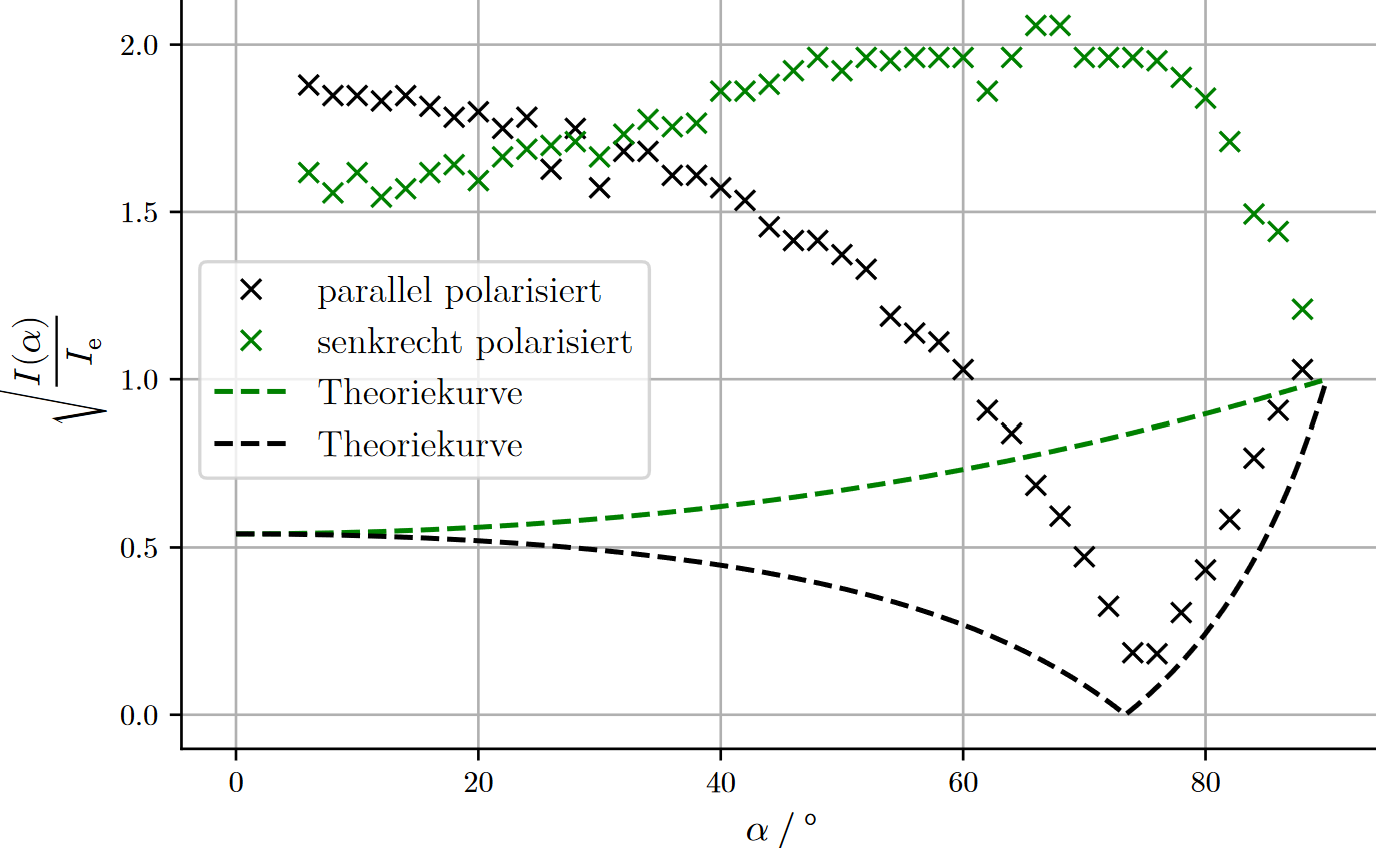
\includegraphics[width=9cm]{plot}
  \caption{Das Verhältnis des reflektierten und einfallenden Stroms gegen den Winkel.}
  \label{plot}
\end{figure}
Aus dem Plot und aus den Messwerten in \autoref{sec:a} ist erkennbar, das der Brewsterwinkel bei ungefähr $\alpha_p=73^\circ$ liegt. Mit \eqref{eq:3} ergibt sich 
\begin{equation*}
  n=3.27
\end{equation*}
für den Brechungsindex von Silizium bei Licht mit der Wellenlänge $\lambda=633\ \textrm{nm}$.
